% Options for packages loaded elsewhere
% Options for packages loaded elsewhere
\PassOptionsToPackage{unicode}{hyperref}
\PassOptionsToPackage{hyphens}{url}
\PassOptionsToPackage{dvipsnames,svgnames,x11names}{xcolor}
%
\documentclass[
  11pt,
]{article}
\usepackage{xcolor}
\usepackage[margin=1in]{geometry}
\usepackage{amsmath,amssymb}
\setcounter{secnumdepth}{-\maxdimen} % remove section numbering
\usepackage{iftex}
\ifPDFTeX
  \usepackage[T1]{fontenc}
  \usepackage[utf8]{inputenc}
  \usepackage{textcomp} % provide euro and other symbols
\else % if luatex or xetex
  \usepackage{unicode-math} % this also loads fontspec
  \defaultfontfeatures{Scale=MatchLowercase}
  \defaultfontfeatures[\rmfamily]{Ligatures=TeX,Scale=1}
\fi
\usepackage{lmodern}
\ifPDFTeX\else
  % xetex/luatex font selection
  \setmainfont[]{Georgia}
\fi
% Use upquote if available, for straight quotes in verbatim environments
\IfFileExists{upquote.sty}{\usepackage{upquote}}{}
\IfFileExists{microtype.sty}{% use microtype if available
  \usepackage[]{microtype}
  \UseMicrotypeSet[protrusion]{basicmath} % disable protrusion for tt fonts
}{}
\makeatletter
\@ifundefined{KOMAClassName}{% if non-KOMA class
  \IfFileExists{parskip.sty}{%
    \usepackage{parskip}
  }{% else
    \setlength{\parindent}{0pt}
    \setlength{\parskip}{6pt plus 2pt minus 1pt}}
}{% if KOMA class
  \KOMAoptions{parskip=half}}
\makeatother
% Make \paragraph and \subparagraph free-standing
\makeatletter
\ifx\paragraph\undefined\else
  \let\oldparagraph\paragraph
  \renewcommand{\paragraph}{
    \@ifstar
      \xxxParagraphStar
      \xxxParagraphNoStar
  }
  \newcommand{\xxxParagraphStar}[1]{\oldparagraph*{#1}\mbox{}}
  \newcommand{\xxxParagraphNoStar}[1]{\oldparagraph{#1}\mbox{}}
\fi
\ifx\subparagraph\undefined\else
  \let\oldsubparagraph\subparagraph
  \renewcommand{\subparagraph}{
    \@ifstar
      \xxxSubParagraphStar
      \xxxSubParagraphNoStar
  }
  \newcommand{\xxxSubParagraphStar}[1]{\oldsubparagraph*{#1}\mbox{}}
  \newcommand{\xxxSubParagraphNoStar}[1]{\oldsubparagraph{#1}\mbox{}}
\fi
\makeatother


\usepackage{longtable,booktabs,array}
\usepackage{calc} % for calculating minipage widths
% Correct order of tables after \paragraph or \subparagraph
\usepackage{etoolbox}
\makeatletter
\patchcmd\longtable{\par}{\if@noskipsec\mbox{}\fi\par}{}{}
\makeatother
% Allow footnotes in longtable head/foot
\IfFileExists{footnotehyper.sty}{\usepackage{footnotehyper}}{\usepackage{footnote}}
\makesavenoteenv{longtable}
\usepackage{graphicx}
\makeatletter
\newsavebox\pandoc@box
\newcommand*\pandocbounded[1]{% scales image to fit in text height/width
  \sbox\pandoc@box{#1}%
  \Gscale@div\@tempa{\textheight}{\dimexpr\ht\pandoc@box+\dp\pandoc@box\relax}%
  \Gscale@div\@tempb{\linewidth}{\wd\pandoc@box}%
  \ifdim\@tempb\p@<\@tempa\p@\let\@tempa\@tempb\fi% select the smaller of both
  \ifdim\@tempa\p@<\p@\scalebox{\@tempa}{\usebox\pandoc@box}%
  \else\usebox{\pandoc@box}%
  \fi%
}
% Set default figure placement to htbp
\def\fps@figure{htbp}
\makeatother





\setlength{\emergencystretch}{3em} % prevent overfull lines

\providecommand{\tightlist}{%
  \setlength{\itemsep}{0pt}\setlength{\parskip}{0pt}}



 


\makeatletter
\@ifpackageloaded{caption}{}{\usepackage{caption}}
\AtBeginDocument{%
\ifdefined\contentsname
  \renewcommand*\contentsname{Table of contents}
\else
  \newcommand\contentsname{Table of contents}
\fi
\ifdefined\listfigurename
  \renewcommand*\listfigurename{List of Figures}
\else
  \newcommand\listfigurename{List of Figures}
\fi
\ifdefined\listtablename
  \renewcommand*\listtablename{List of Tables}
\else
  \newcommand\listtablename{List of Tables}
\fi
\ifdefined\figurename
  \renewcommand*\figurename{Figure}
\else
  \newcommand\figurename{Figure}
\fi
\ifdefined\tablename
  \renewcommand*\tablename{Table}
\else
  \newcommand\tablename{Table}
\fi
}
\@ifpackageloaded{float}{}{\usepackage{float}}
\floatstyle{ruled}
\@ifundefined{c@chapter}{\newfloat{codelisting}{h}{lop}}{\newfloat{codelisting}{h}{lop}[chapter]}
\floatname{codelisting}{Listing}
\newcommand*\listoflistings{\listof{codelisting}{List of Listings}}
\makeatother
\makeatletter
\makeatother
\makeatletter
\@ifpackageloaded{caption}{}{\usepackage{caption}}
\@ifpackageloaded{subcaption}{}{\usepackage{subcaption}}
\makeatother
\usepackage{bookmark}
\IfFileExists{xurl.sty}{\usepackage{xurl}}{} % add URL line breaks if available
\urlstyle{same}
\hypersetup{
  pdftitle={Does Restricting Airbnb Lower Rents?},
  pdfauthor={John Scheble},
  colorlinks=true,
  linkcolor={black},
  filecolor={Maroon},
  citecolor={Blue},
  urlcolor={blue},
  pdfcreator={LaTeX via pandoc}}


\title{Does Restricting Airbnb Lower Rents?}
\usepackage{etoolbox}
\makeatletter
\providecommand{\subtitle}[1]{% add subtitle to \maketitle
  \apptocmd{\@title}{\par {\large #1 \par}}{}{}
}
\makeatother
\subtitle{Estimating Effects from NYC's Local Law 18}
\author{John Scheble}
\date{2026-07-07}
\begin{document}
\maketitle


New York City's housing market has faced a prolonged affordability
crisis, with median rents rising sharply over the past decade and rental
vacancy rates hovering near historic lows. One frequently cited reason
for this pressure is the rapid growth of short-term rental platforms
like Airbnb, which critics argue pull units out of the long-term rental
market and drive up rents for permanent residents. This study attempts
to quantify that relationship by evaluating whether the enforcement of
Local Law 18, NYC's landmark short-term rental regulation, had a
measurable dampening effect on rent prices across the city's zip codes.

Local Law 18 was passed by the NYC City Council in January 2022 and
signed into law shortly after. Enforcement began on September 5, 2023,
making New York City one of the strictest short-term rental markets in
the world. The law requires all short-term rental hosts to register with
the Mayor's Office of Special Enforcement, mandates that the host be
physically present during any guest stay, and caps occupancy at two
guests per rental.

\subsection{Data}\label{data}

The data used in this analysis comes from three main sources: Zillow,
the U.S. Census Bureau, and Inside Airbnb. Zillow provides the Zillow
Observed Rent Index (ZORI), a measure of median rent prices in various
geographic areas; I obtained ZORI data for all New York City zip codes
from January 2015 to December 2025. Housing unit counts used to
normalize Airbnb activity were collected from Census data. Inside Airbnb
is a third-party data source that scrapes Airbnb and provides
information on all active listings at the time of the scrape. Earlier
snapshots exist and are documented, but aren't yet incorporated into
this model; as a result, this analysis should be understood to carry
some degree of survivorship bias in its listing counts, likely
undercounting true activity levels.

\begin{figure}[H]

{\centering \pandocbounded{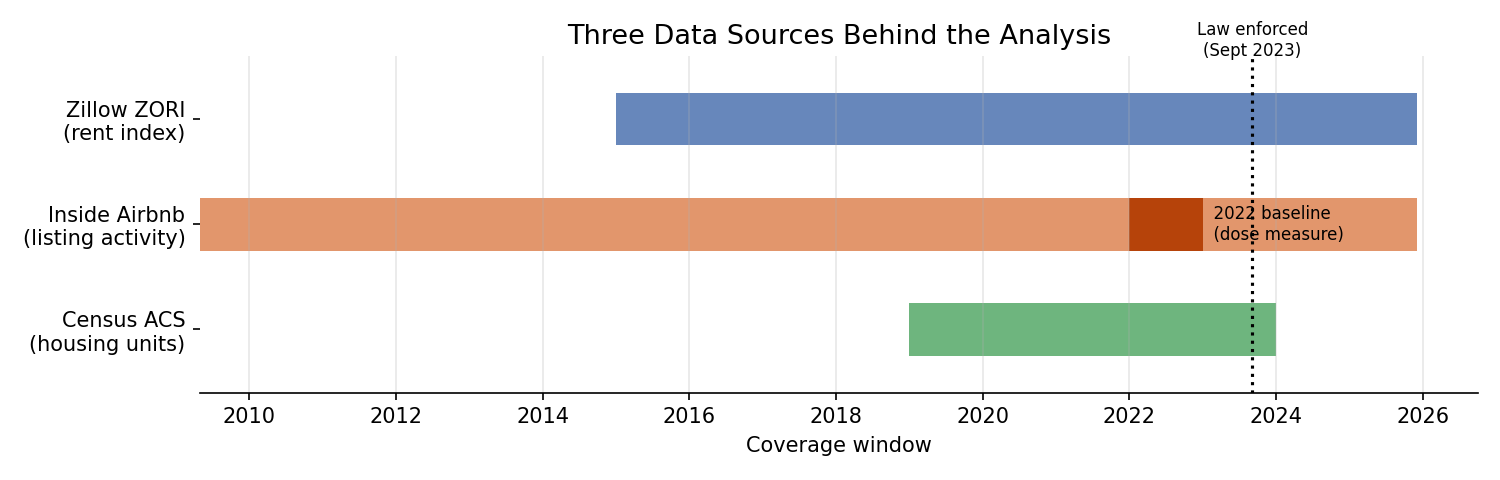
\includegraphics[keepaspectratio]{data_sources_timeline.png}}

}

\caption{Coverage windows for the three data sources behind the
analysis. The 2022 baseline window (dark orange) is the period used to
construct the Airbnb intensity measure.}

\end{figure}%

\subsection{Method}\label{method}

To isolate the law's effect, I compared rent trends in zip codes with
heavy Airbnb activity to trends in zip codes with little to none, before
and after enforcement began in September 2023. This is a
difference-in-differences approach that's commonly used to isolate an
effect from a change in the law alone. I also controlled for fixed
differences between zip codes and across months, to ensure normal
neighborhood and seasonal changes wouldn't affect the results. A key
assumption underlying the analysis was that, absent the law affecting
Airbnb activity, high- and low-Airbnb zip codes would have kept moving
in roughly the same direction. This assumption was found to be incorrect
quickly.

\subsection{Results}\label{results}

My baseline model comparing rent trends in high- and low-Airbnb zip
codes before and after Local Law 18 found no statistically significant
effect (p = 0.75). That result is difficult to interpret on its own,
however. In reality, zip codes with the most Airbnb activity were
already on a different rent trajectory before the law took effect,
driven in large part by the uneven COVID-era rent crash and rebound in
neighborhoods like lower Manhattan and North Brooklyn.

Once that pre-existing divergence between zip codes' rent trajectories
is accounted for, the model finds a negative association between Airbnb
intensity and rent growth (0.3--0.65\% per unit of Airbnb intensity,
95\% confidence interval). This implies the law acted as a mild
rent-suppressing effect, concentrated in the highest-intensity
neighborhoods.

\begin{figure}[H]

{\centering \pandocbounded{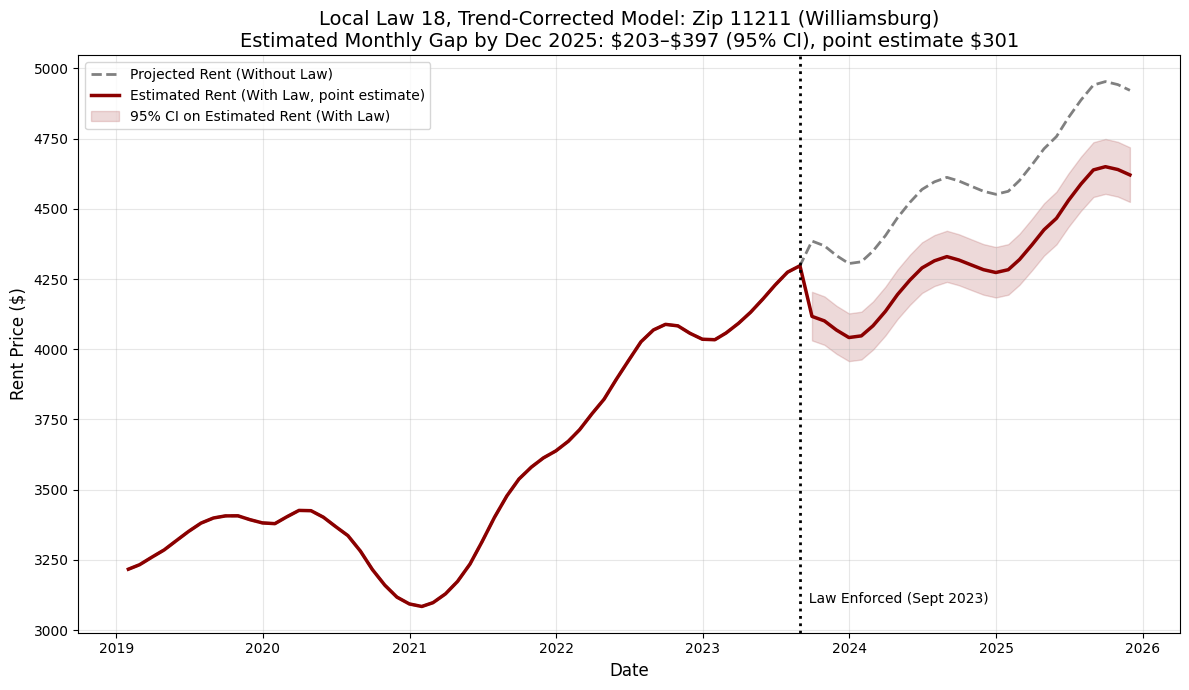
\includegraphics[keepaspectratio]{williamsburg_case_study.png}}

}

\caption{Local Law 18's trend-corrected effect in Williamsburg (zip
11211), the highest-intensity zip code in the sample. The shaded band
reflects the 95\% confidence interval on the estimated effect, not a
point-estimate claim.}

\end{figure}%

That said, this corrected estimate should be read as suggestive rather
than conclusive. The correction technique I used, a zip-specific time
trend, is a standard tool, but it's unable to fully separate the law's
effect from COVID-era rent dynamics cooling off on their own. They both
predict the same pattern in the data, and the two are difficult to fully
disentangle. The Airbnb-activity measure used here is also likely to
undercount listings that were removed by the law itself, which could
bias the estimated effect in either direction. Addressing the
data-quality issue using archival listing snapshots, and applying more
formal sensitivity-bound methods to test how much the result depends on
the parallel-trends assumption, is the next phase of this project.

\subsection{Conclusion}\label{conclusion}

Taken together, the evidence is consistent with Local Law 18 having
modestly slowed rent growth in the highest-Airbnb-density neighborhoods,
but the magnitude of that effect is hard to quantify with certainty, and
a more definitive answer requires a larger dataset and more rigorous
testing.




\end{document}
